\section{Hoja 1: Integración numérica}

Para el apartado de integración numérica se han implementado los métodos del rectángulo (por la derecha, izquierda y punto medio), del trapecio y de Simpson.

\begin{lstlisting}[language=Matlab, caption={Fórmulas de integración.},captionpos=b,texcl=true]
function res = rectanguloA(f,a,b) % Rectángulo izquierda.
    res = f(a)*(b-a);
end

function res = rectanguloB(f,a,b) % Rectángulo derecha.
    res = f(b)*(b-a);
end

function res = rectanguloAB(f,a,b) % Rectángulo punto medio.
    res = f((a+b)/2)*(b-a);
end

function res = trapecio(f,a,b) % Fórmula del Trapecio
    res = ((b-a)/2)*(f(a)+f(b));
end

function res = simpson(f,a,b) % Fórmula de Simpson 1/3 
    res = (b-a)*(f(a)+4*f((a+b)/2)+f(b))*1/6;
end
\end{lstlisting}

Adicionalmente se ha implementado una función de \textit{Matlab} que recibe como parámetros la función a integrar, una referencia al método y una lista de puntos en el eje X que servirán de intervalos.

\begin{lstlisting}[language=Matlab, caption={Función que aplica el método de integración en los intervalos.},captionpos=b,texcl=true]
% Para aplicar diversos métodos en el apartado B
function res = aplicarMetodo(func, met, X)
    res = 0;
    for i = 1:length(X)-1
        res = res + met(func, X(i), X(i+1));
    end
end
\end{lstlisting}

\subsection{Apartado A}
Aplicamos los métodos al cálculo de \(\int_{0}^{1} e^x \,dx\) y los comparamos con el valor exacto computado con:
\begin{lstlisting}
fA=@(x) exp(x);
exactoA = integral(fA,0,1); % valor exacto e^x en [0,1]
\end{lstlisting}

Podemos apreciar que el incremento en el número de intervalos aproxima el resultado a la solución exacta usando el mismo método y que, comparando la solución de cada método con el mismo número de intervalos (1000 en nuestro caso) con el valor exacto, vemos que el error cometido es mucho menor con la fórmula de Simpson que aproxima cuadráticamente (ver \autoref{tbl:errorIntA}). Una gráfica de la disminución del error puede verse en la \autoref{errorIntFig}.
\begin{table}
\begin{center}
\begin{tabular}{ |c|c| } 
 \hline 
 Metodo & abs(exacto-resultado) \\ 
 \hline \hline
 Rectángulo izquierda &  $8.59\times10^{-04}$ \\ 
 \hline
 Rectángulo derecha &  $8.59\times10^{-04}$ \\ 
 \hline
 Rectángulo punto medio &  $7.16\times10^{-08}$ \\ 
 \hline
 Trapecio &  $1.4319\times10^{-07}$ \\ 
 \hline
 Simpson &  $1.9984\times10^{-15}$ \\ 
 \hline
\end{tabular}
\end{center}
\caption{Error absoluto cometido para el apartado A con 1000 intervalos.}
\label{tbl:errorIntA}
\end{table}

\begin{figure}[!h]
  \centering
  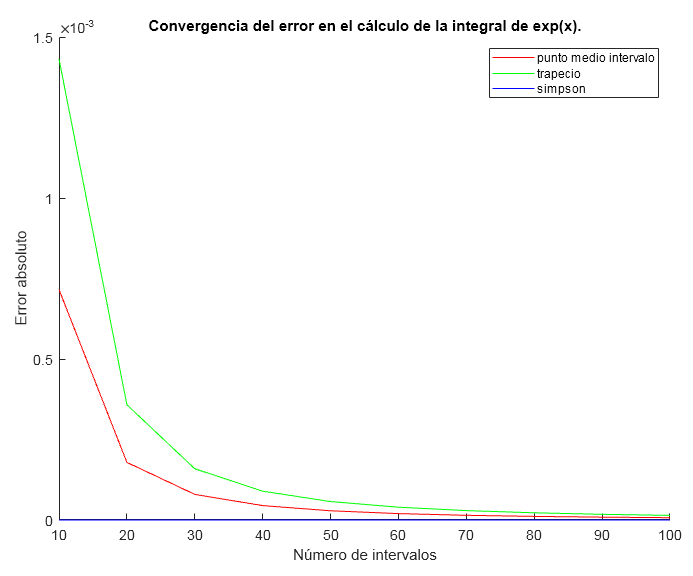
\includegraphics[width=\linewidth]{Integracion/error_int.png}
  \caption{Disminución del error al aumentar el número de intervalos (no se incluyen métodos con un error mayor).}
  \label{errorIntFig}
\end{figure}

\subsection{Apartado B}
Aplicamos los métodos al cálculo de \(\int_{0}^{2\pi} cos(x^2 - 1) \,dx\) y los comparamos con el valor exacto y la aproximación computados con:
\begin{lstlisting}
fB=@(x) cos((x.^2) - 1);
X = 0:pi/1000:2*pi;
Y = arrayfun(fB,X);
aproxiB = trapz(X,Y);
exactoB = integral(fB, 0, 2*pi);
\end{lstlisting}

Usando esta vez 2000 intervalos obtenemos unas conclusiones similares al apartado A (ver \autoref{tbl:errorIntB}).
\begin{table}
\begin{center}
\begin{tabular}{ |c|c| } 
 \hline 
 Metodo & abs(exacto-resultado) \\ 
 \hline \hline
 Rectángulo izquierda &  $2.7603\times10^{-04}$ \\ 
 \hline
 Rectángulo derecha &  $2.615\times10^{-04}$ \\ 
 \hline
 Rectángulo punto medio &  $3.632\times10^{-06}$ \\ 
 \hline
 Trapecio &  $7.2638\times10^{-06}$ \\ 
 \hline
 Simpson &  $4.5356\times10^{-11}$ \\ 
 \hline
\end{tabular}
\end{center}
\caption{Error absoluto cometido para el apartado B con 2000 intervalos.}
\label{tbl:errorIntB}
\end{table}

No se incluye la gráfica del error en el caso del apartado B por ser muy similar a la ya mostrada en el apartado A con el mismo incremento en el número de intervalos.